\section{Workflow Abstraction}

\label{sec:abstraction}
% Is having the trie structure the objective behing workflow abstraction? 
% I would have imagined that it is more about enabling reuse, discovery of 
% workflows and so on. -- khalid
% I would use the above paragraph in the beginning for the reader to 
% understand what the rational behind workflow abstraction is. -- khalid

% I moved this paragraph here for better understanding as suggested
%	--Esteban.

The goal of specifying the abstraction of a workflow is to make workflows more reusable as a whole or some parts of it. In our work we define abstraction as the pattern that appears when a sequence of resources are executed together by a minimum number of times. This definition leads also to the concept of pattern or macro identification which applied to workflows leads to finding common sub-workflows. The work done so far for this purpose has been the creation of a trie structure~\cite{knuth11} which captures the sequences of execution of a workflow and keeps track of their statistics. 


\subsection{Workflow abstraction discovery process}
Figure~\ref{fig:workflowAbstraction} shows the overall discovery process introduced in this section. The inputs are obtained by using the provenance of workflow results~\footnote{\url{http://wf4ever.github.com/ro-primer/}} from WINGS and Taverna. That provenance is stored in a trie structure which captures the order of the executed resources and stores the frequencies of appearance. Then, that information can be used to obtain the most frequent set of ordered executed resources which we have called macros and are identified in the figure at the bottom by black squares. Afterwards these detected macros, which represent some common workflow structures, could be hand-annotated in order to tag them or could be annotated automatically for example by assigning to them the same tags as the workflows that they belong to. Finally a taxonomy which includes all the identified macros by membership (bigger macros contain the smaller ones) can be created for indexing.
% The above paragraph may be more useful in the beginning to illustrate 
% to the user the approach, before starting the discussion of Trie 
% structure. -- khalid

\subsection{Trie structure to store the provenance of workflow results}
As introduced above we have used a trie for storing the workflow execution in an ordered way by including at different levels of depth the different inputs, processes and outputs (resources) which have been executed. A trie is defined as an ordered tree that stores a dynamic set of keys which are allocated at the leafs and the different internal nodes are the gateways. Therefore all the descendants of a node have a common prefix of the resource associated with that node. This is very useful for detecting common parts of different workflows because we can easily keep track of the number of times that a specific sequence of resources has been executed.

Therefore, the presented work is a bottom-up approach in order to study the actual provenance of workflow results (which represents the dataflow of an executed workflow as described in D4.2v1~\cite{D4.2v1}) from a set of available workflows at WINGS~\footnote{\url{http://wings.isi.edu/}} and Taverna~\footnote{\url{http://www.taverna.org.uk/}} created for this purpose. The definition of the provenance of workflow results and \textbf{wfprov} ontology are available at~\footnote{\url{http://wf4ever.github.com/ro-primer/}} and \footnote{\url{http://purl.org/wf4ever/wfprov}} respectively, and some examples which have been created for this work and are part of the RO testbed \footnote{\url{http://www.wf4ever-project.org/wiki/display/docs/RO+testbed}}. The provenance of the workflow results of the different workflows examples have been used as inputs for creating the trie structure introduced above. Every resource executed and capture by the \textbf{wfprov} of a RO is then associated to a node in the trie structure and its frequency updated by increasing the number of times that it has appeared. Afterwards an analysis of the trie is done to obtain the most common set of resources which are going to identify the pursued abstract macros. \\

% I think that an example that shows a workflow and a corresponding true 
% structure would be helpful for teh reader to understand what it is about. 
% -- khalid
% The work main purpose is to detect those patterns from examples this is the reason why
% I do not see how to show an specific case.
%	--Esteban

% How is the information about the number of executing a given resource
% important for workflow abstraction? -- khalid
 
Although this is still a preliminary work and more examples are needed in order to be able to extract relevant macros, once a set of macros have been identified it would be possible to categorize them (manually or automatically e.g. by using workflow tags) and then build the associated taxonomy by using the trie membership relations. The code developed for the creation and maintenance of the trie structure and for accessing to the provenance of the workflow results repository is available at \footnote{\url{https://github.com/wf4ever/wf-abstraction}} and provides the following functionality:
\begin{itemize}
\item It stores the provenance of the workflow results in an ordered way and the appearance frequency of their resources
\item It calculates relative frequencies at different levels of the trie
\item It provides different modes to traverse the structure (pre-ordered/level-ordered)
\item It provides an output XML structure with relative frequencies per level and per process (an output example is available at \footnote{\url{https://github.com/wf4ever/wf-abstraction/blob/master/outputExample.xml})}
\end{itemize}





%The use of the provenance of the workflow results seems to be more appealing that using the workflow templates, which are the static description %of a workflow, mainly due to it representing the workflows which are actually running and being used, and also allows to undo control structures %as e.g. "if".
% Scientific workflows such as Taverna and Wings do not have 
% control based flows such as If. Do you intend to support
% workflow system that do? If yesm it would be good to specify which 
% the ones. -- khalid
% Not sure if Galaxy has it so I deleted the sentece.
%	--Esteban




\begin{figure}
\begin{center}
	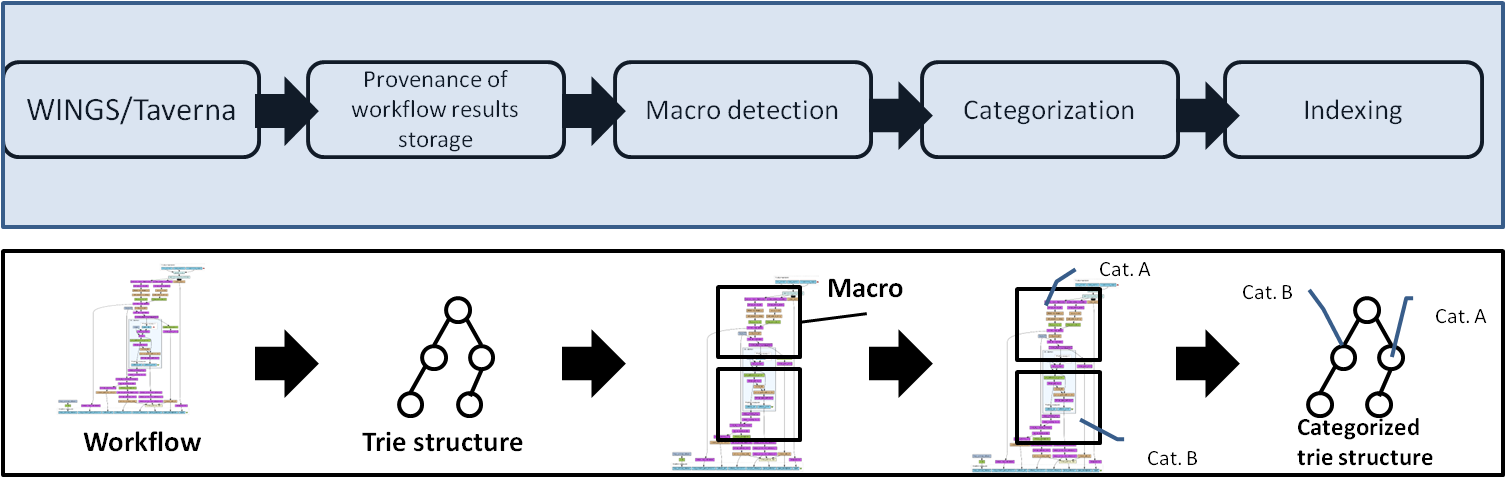
\includegraphics[scale=0.65]{./Figures/workflowAbstraction}
		\caption{Workflow abstraction discovery process.}
		\label{fig:workflowAbstraction}
\end{center}
\end{figure}
% according to Kevin, the above Figure is still small.
% It may be worth having redesigning it to have the steps go through
% Verticallym instead of horizontally, as this will give you more space 
% to illustrate them. -- khalid
% I made it bigger
%	--Esteban.